% ------------------------------------------------------------------------------
% TYPO3 CMS 7.6 - What's New (English Version)
%
% @author	Patrick Lobacher <patrick@lobacher.de> and Michael Schams <schams.net>
% @license	Creative Commons BY-NC-SA 3.0
% @link		http://typo3.org/download/release-notes/whats-new/
% @language	English
% ------------------------------------------------------------------------------
% LTXE-CHAPTER-UID:		d71b4b88-f79b2343-d2b356bf-452cef81
% LTXE-CHAPTER-NAME:	Backend User Interface
% ------------------------------------------------------------------------------

\section{Backend User Interface}
\begin{frame}[fragile]
	\frametitle{Backend User Interface}

	\begin{center}\huge{Chapter 1:}\end{center}
	\begin{center}\huge{\color{typo3darkgrey}\textbf{Backend User Interface}}\end{center}

\end{frame}

% ------------------------------------------------------------------------------
% LTXE-SLIDE-START
% LTXE-SLIDE-UID:		d8599a04-11b4fa8c-9be5812a-715820e1
% LTXE-SLIDE-ORIGIN:	ef1d6d8c-0db67396-dedb5814-1767169f German
% LTXE-SLIDE-TITLE:		Rework workspace notification settings (1)
% LTXE-SLIDE-REFERENCE:	Feature-35245-ReworkWorkspaceNotificationSettings.rst
% ------------------------------------------------------------------------------
\begin{frame}[fragile]
	\frametitle{Backend User Interface}
	\framesubtitle{Workspaces Notification Settings (1)}

	Meaning and behavior of notification settings have been streamlined\newline
	\smaller(an upgrade wizard helps to upgrade the settings to the new definitions)\normalsize

	\begin{figure}
		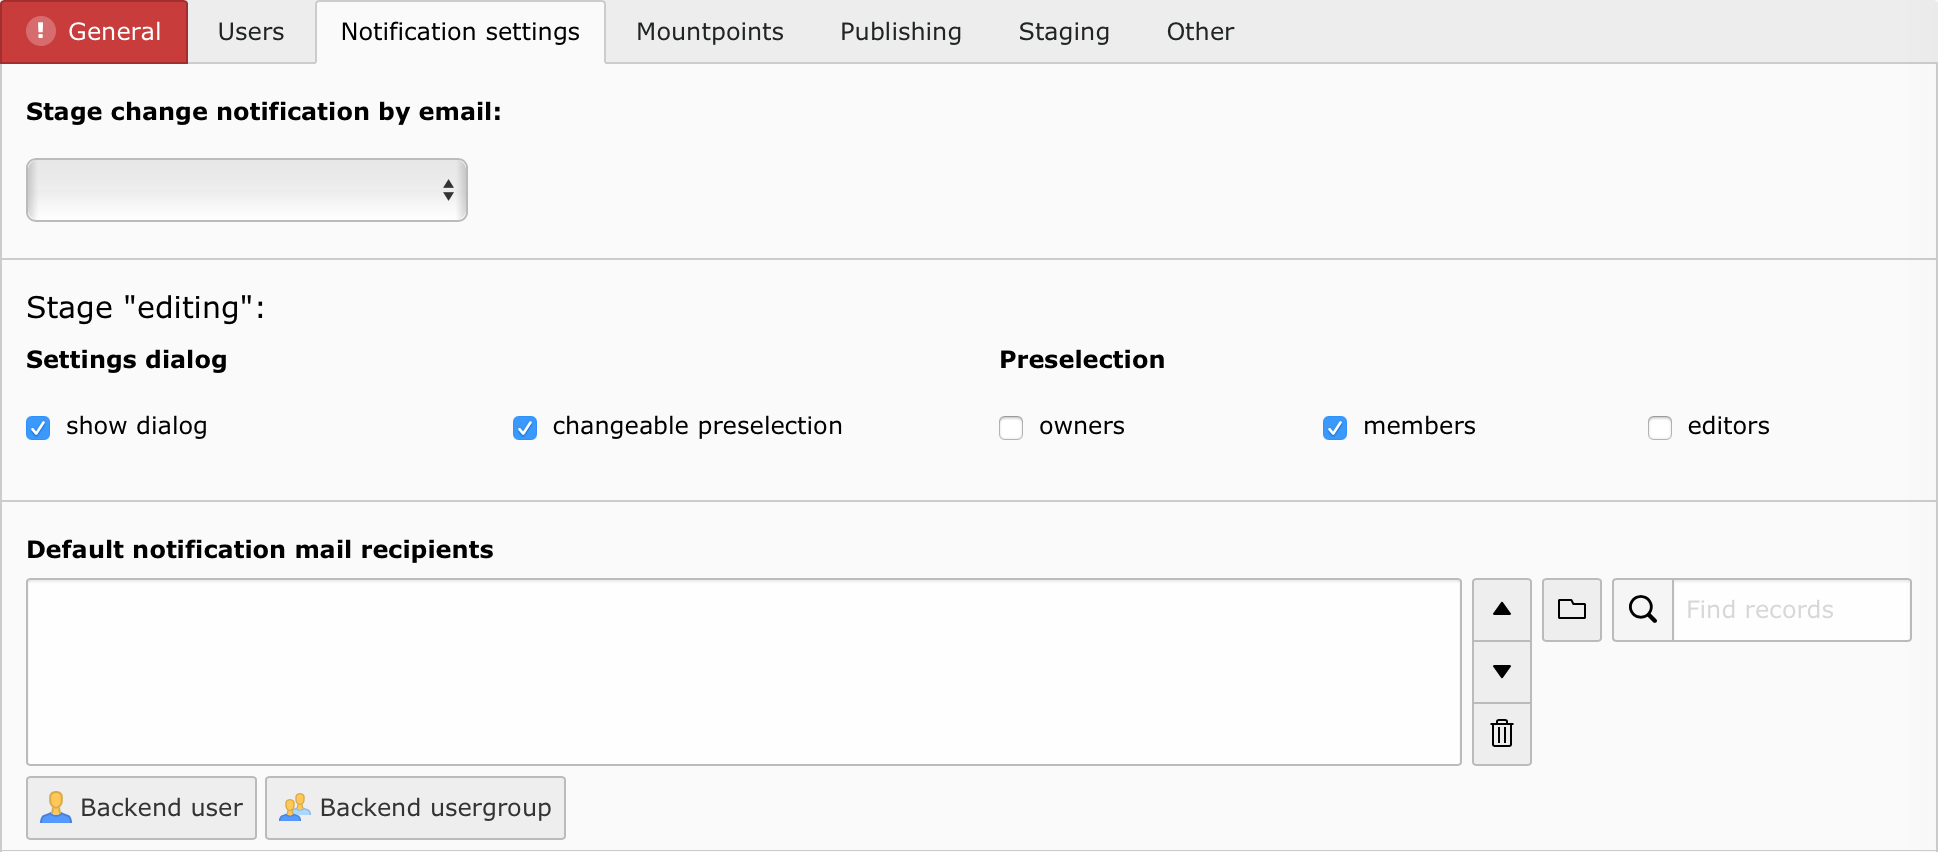
\includegraphics[width=0.94\linewidth]{BackendUserInterface/35245a.png}
	\end{figure}

\end{frame}

% ------------------------------------------------------------------------------
% LTXE-SLIDE-START
% LTXE-SLIDE-UID:		04855567-dac16e24-f5274c64-f1d49c36
% LTXE-SLIDE-ORIGIN:	1db1430d-4db24c16-2bf357bb-5f5c85db German
% LTXE-SLIDE-TITLE:		Rework workspace notification settings (2)
% LTXE-SLIDE-REFERENCE:	Feature-35245-ReworkWorkspaceNotificationSettings.rst
% ------------------------------------------------------------------------------
\begin{frame}[fragile]
	\frametitle{Backend User Interface}
	\framesubtitle{Workspaces Notification Settings (2)}

	Stage \textbf{publishing execute} received configuration options

	\begin{figure}
		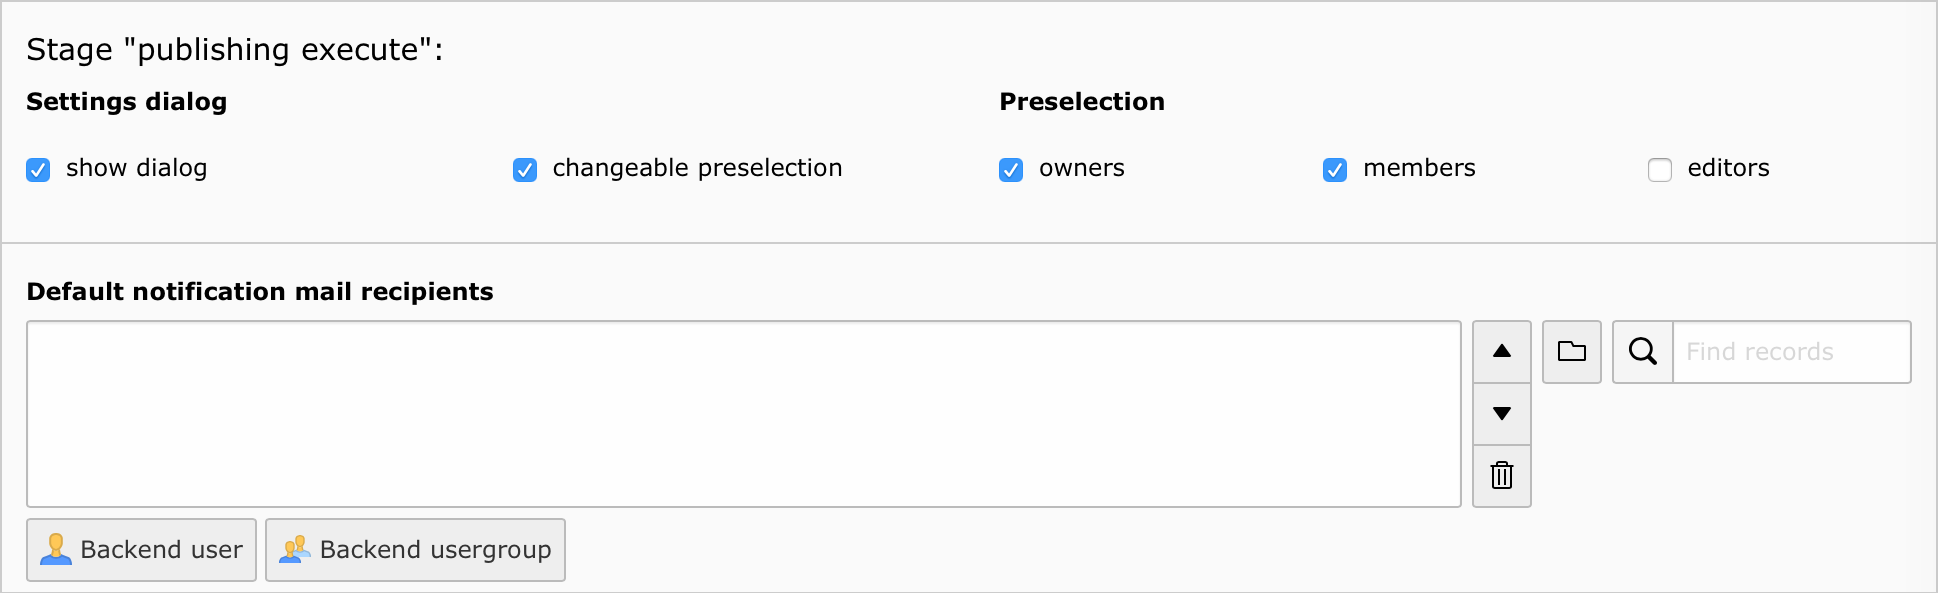
\includegraphics[width=0.94\linewidth]{BackendUserInterface/35245b.png}
	\end{figure}

\end{frame}

% ------------------------------------------------------------------------------
% LTXE-SLIDE-START
% LTXE-SLIDE-UID:		fd6d762a-b268caf0-cb6f9195-f553e035
% LTXE-SLIDE-ORIGIN:	80fbd7db-2c4c98db-06e09bb9-ef0a5112 German
% LTXE-SLIDE-TITLE:		Add basic file search in element browser
% LTXE-SLIDE-REFERENCE:	Feature-69120-AddBasicFileSearchInElementBrowser.rst
% ------------------------------------------------------------------------------
\begin{frame}[fragile]
	\frametitle{Backend User Interface}
	\framesubtitle{Search Functionality in Element Browser}

	File search has been added to the TYPO3 Element Browser (works recursively)

	\begin{figure}
		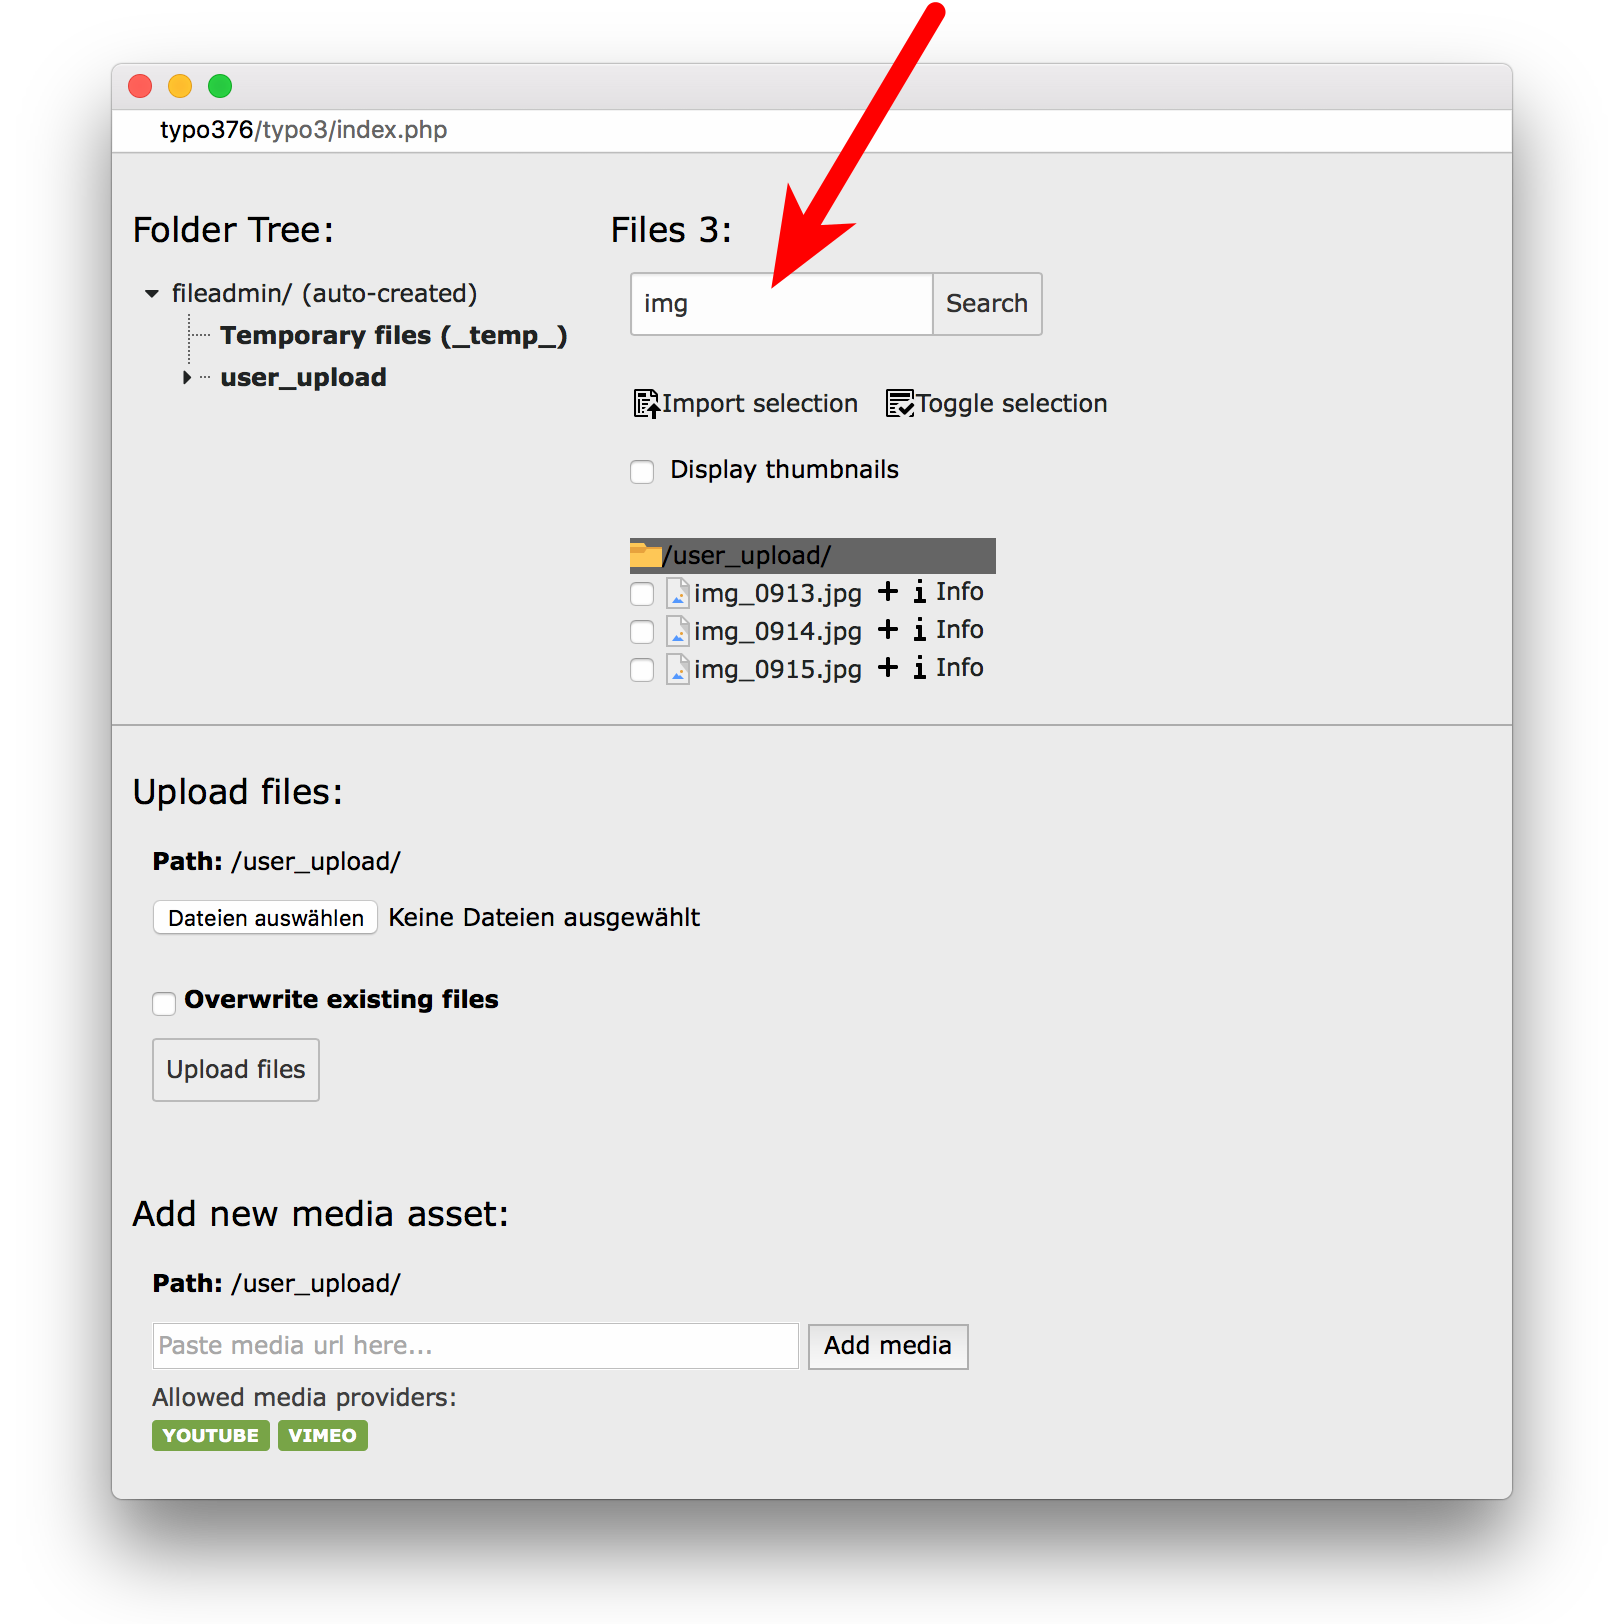
\includegraphics[width=0.4\linewidth]{BackendUserInterface/69120.png}
	\end{figure}

\end{frame}

% ------------------------------------------------------------------------------
